\section{Planarität testen}

\textbf{Problem}: Gegeben ein Graph $G$ als Adjazenzliste, entscheide ob $G$ planar ist

\textbf{Möglichkeit}: 
\begin{itemize}
	\item Teste auf $K_5$- oder $K_{3,3}$-Unterteilung
	\item Es existiert ein theoretisch effizienter, aber nicht praktikabler Algorithmus dafür, da die Laufzeit sehr groß werden kann
	\item Im Folgenden: \textbf{LR-Planarität}
\end{itemize}

\textbf{Annahmen}:
\begin{itemize}
	\item $G$ hat keine Mehrfachkante
	\item $G$ hat keine Schlingen
	\item $G$ hat keine Brücken, also liegt jede Kante auf einem Kreis
	\item $G$ ist zusammenhängend
\end{itemize}

\textbf{Vorbereitendes Vorgehen}:
\begin{itemize}
	\item Tiefensuche von beliebigem Startknoten
	\item Nummeriere Knoten in Explorierungsreihenfolge
	\item Orientiere Baumkanten in Explorierungsreihenfolge und Nichtbaumkanten vom Knoten mit größerer DFS-Zahl zum Knoten mit kleinerer DFS-Zahl
	\begin{center}
		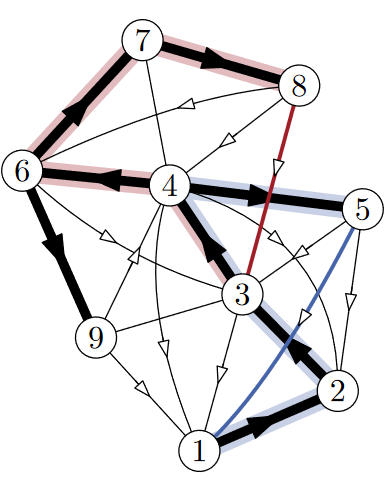
\includegraphics[width=0.2\textwidth]{images/dfs.png}
	\end{center}
\end{itemize}

\textbf{Erste Beobachtungen}:
\begin{itemize}
	\item Nichtbaumkanten verbinden immer zwei Knoten auf einem Wurzel-Blatt-Pfad.
	\item Jede Nichtbaumkante $e$ schließt einen eindeutigen Kreis mit den Baumkanten (\textbf{Fundamentalkreis} zu $e$).
	\item Jede planare Zeichnung von $G$ liefert auch eine planare Zeichnung des DFS-Baums. Betrachte Zeichnung mit der Wurzel an der äußeren Facette.
	\item Jede Nichtbaumkante $e$ führt entweder links (\textbf{$\mathbf{L}$-Kante}) oder rechts (\textbf{$\mathbf{R}$-Kante}) am Baum zurück.
	\item Um herauszufinden, ob $G$ planar ist, müssen wir entweder eine Einteilung der Nichtbaumkanten in $L$- und $R$-Kanten finden bei der keine Überschneidungen entstehen (\textbf{LR-Zerlegung}) oder zeigen, dass eine solche Einteilung nicht existiert.
\end{itemize}
\bigskip
\textbf{Definition}: Sei $e$ eine Kante. Eine Nichtbaumkante $(x, y)$ heißt \textbf{Rückkante} von $e$, wenn $e$ auf dem Fundamentalkreis von $(x, y)$ liegt. Dann nennt man $y$ einen \textbf{Rückkehrpunkt} von $e$. Ist $e$ eine Nichtbaumkante, so ist $e$ seine einzige und eigene Rückkante mit eindeutigem Rückkehrpunkt.
\begin{center}
	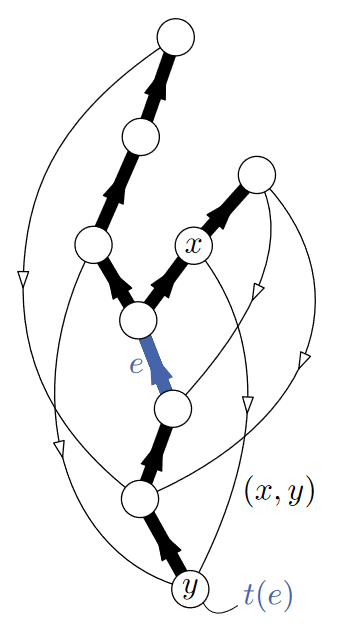
\includegraphics[width=0.2\textwidth]{images/back-edge.png}
\end{center}

\textbf{Definition}: Sei $e$ eine Kante. Der tiefste Rückkehrpunkt von $e$
$$t(e)\coloneqq \text{kleinste DFS-Zahl eines Rückkehrpunktes}$$ nennt man den \textbf{Tiefpunkt} von $e$.

\textbf{Definition}: Eine \textbf{Gabel} sind zwei Kanten mit dem gleichen Startpunkt, also $e_1=(u,v_1)$ und $e_2=(u,v_2)$.

\textbf{Definition}: Für eine Gabel $e_1=uv_1$, $e_2=uv_2$ definiere die Mengen
\begin{itemize}
	\item $R(e_1,e_2)\coloneqq\{e \text{ Rückkante von }e_1 \text{ mit }t(e_2)<t(e)<u\}$
	\item $R(e_2,e_1)\coloneqq\{e \text{ Rückkante von }e_2 \text{ mit }t(e_1)<t(e)<u\}$
\end{itemize} 
Zwei Kanten $f_1,f_2$ haben einen \textbf{Konflikt} bezüglich $e_1,e_2$, wenn
\begin{itemize}
	\item $f_1,f_2\in R(e_1,e_2)$ oder $f_1,f_2\in R(e_2,e_1)$ (\textbf{Gleichheitskonflikt})
	\item $f_1 \in R(e_1,e_2)$ und $f_2\in R(e_2,e_1)$ oder umgekehrt (\textbf{Ungleichheitskonflikt})
\end{itemize}
\begin{center}
	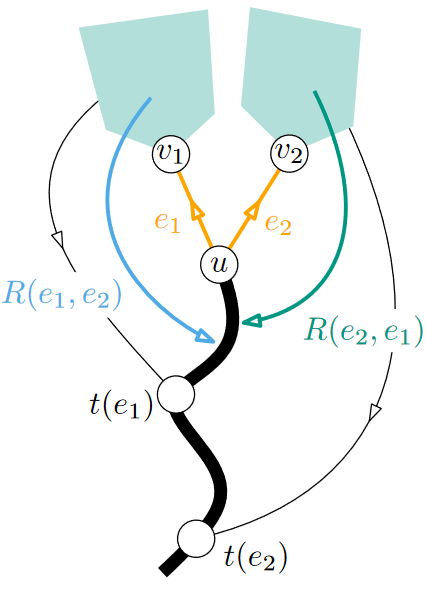
\includegraphics[width=0.25\textwidth]{images/konflikt.png}
\end{center}

\textbf{Definition}: Eine \textbf{LR-Zerlegung} ist eine Partition der Nichtbaumkanten in $L$ und $R$, sodass je zwei Kanten $f_1,f_2$
\begin{itemize}
	\item mit Gleichheitskonflikt in der gleichen Menge sind.
	\item mit Ungleichheitskonflikt in unterschiedlichen Mengen sind.
\end{itemize}
\bigskip
\textbf{Satz}: Folgende Aussagen sind äquivalent:
\begin{itemize}
	\item $G$ ist planar.
	\item Es gibt eine LR-Zerlegung bezüglich einer Tiefensuche.
	\item Es gibt zu jeder Tiefensuche eine LR-Zerlegung
\end{itemize}
\textit{Der Beweis des Satzes wird später skizziert}.\\

\textbf{Planaritätstest basierend auf LR-Zerlegung}
\begin{enumerate}
	\item Tiefensuche auf Graph in $\mathcal{O}(n)=\mathcal{O}(|V(G)|)$
	\item Bestimme naiv alle Kantenkonflikte in $\mathcal{O}(n^2)$, indem man sich z.B. alle Kantenpaare anschaut
	\item Baue Hilfsgraph $H$ mit
	\begin{itemize}
		\item Knoten in $H$ sind Kanten von $G$.
		\item Kanten in $H$ sind Ungleichheitskonflikte in $G$.
		\item Knoten in $H$ werden verschmolzen, wenn sie einen Gleichheitskonflikt haben.
	\end{itemize}
	\begin{center}
		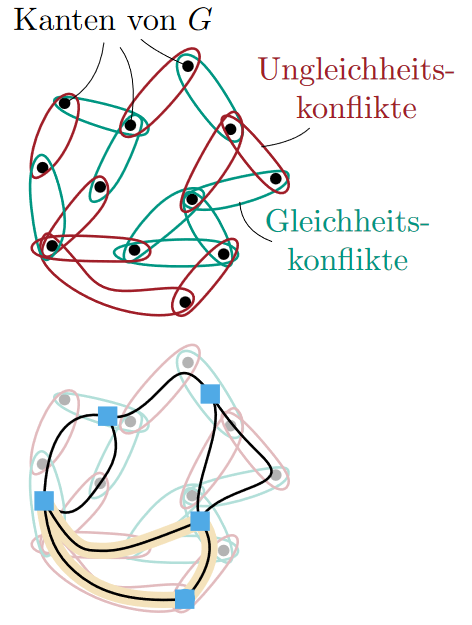
\includegraphics[width=0.25\textwidth]{images/planar-test.png}
	\end{center}
	\item LR-Zerlegung von $G$ existiert $\iff$ $H$ ist bipartit. Teste also den Graphen auf Bipartitheit. Das geht in $\mathcal{O}(n^2)$
\end{enumerate}
$\implies$ Damit haben wir einen Planaritätstest in $\mathcal{O}(n^2)$. Eine Beschleunigung auf $\mathcal{O}(n)$ ist aber möglich.\\

\textit{Korrektheitsbeweis vom obigen Satz}:

Zeige zunächst \underline{$G$ planar $\implies$ $G$ hat LR-Zerlegung}:
\begin{itemize}
	\item Einbettung von $G$ mit Knoten 1 an der äußeren Facette induziert eine Einbettung des gerichteten DFS-Baumes.
	\item Nichtbaumkante $e$ ist in $L$, wenn der Fundamentalkreis zu $e$ gegen den Uhrzeigersinn orientiert ist
	\item Nichtbaumkante $e$ ist in $R$, wenn der Fundamentalkreis zu $e$ im Uhrzeigersinn orientiert ist
	\begin{center}
		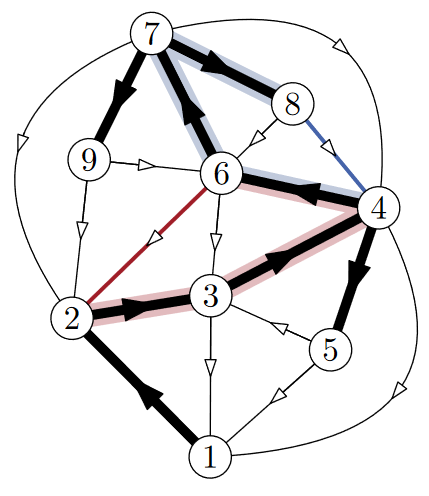
\includegraphics[width=0.15\textwidth]{images/lr-1.png}
	\end{center}
	\item Zeige, dass diese Einteilung in $L$ und $R$ alle Konflikte erfüllt
	\item Betrachte eine Gabel $e_1,e_2$ an Gabelknoten $u$ mit eingehender Baumkante $e$
	\item Seien o.B.d.A. $e, e_1, e_2$ in dieser cw-Reihenfolge um $u$ und $t(e_1)\geq t(e_2)$
	\item Betrachte nun $f_1\in R(e_1,e_2)$ und $f_2\in R(e_2,e_1)$:
	\begin{center}
		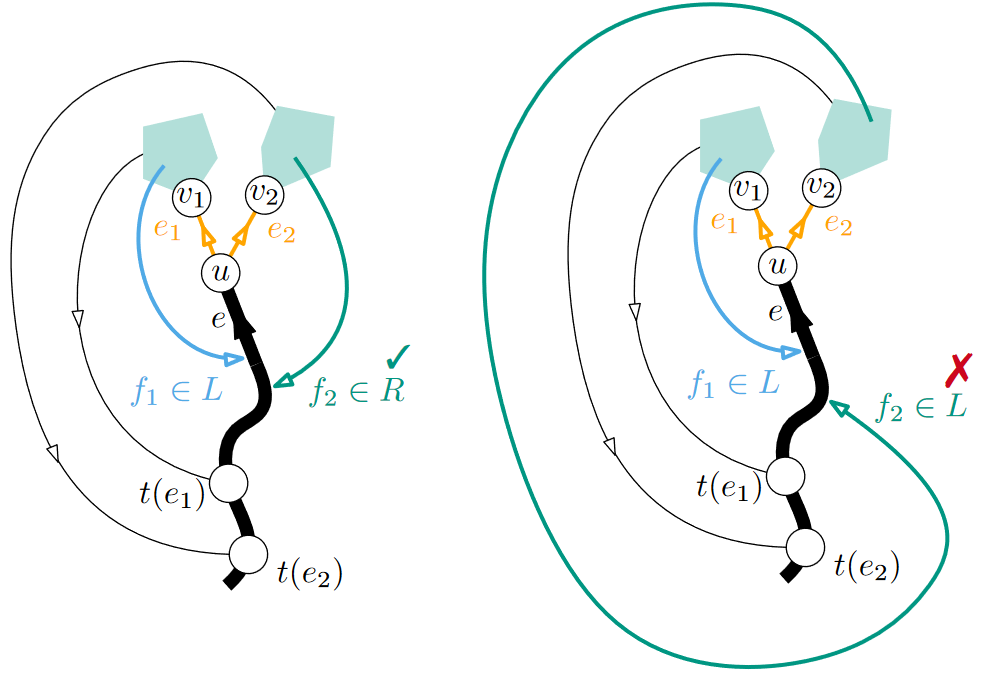
\includegraphics[width=0.45\textwidth]{images/lr-2.png}
	\end{center}
\end{itemize}

Zeige nun \underline{$G$ hat LR-Zerlegung $\implies$ $G$ planar}: 
\begin{itemize}
	\item Betrachte eine LR-Zerlegung, konstruiere eine planare Einbettung von $G$ mit Knoten 1
	an der äußeren Facette, d.h. gib für jeden Knoten die zyklische Reihenfolge der inzidenten Kanten an
\end{itemize}

\textbf{Schritt 1}: LR-Zerlegung bündeln
\begin{itemize}
	\item Eine LR-Zerlegung heißt \textbf{gebündelt} wenn zu jeder Kante $e$ alle Rückkanten von $e$ mit Rückkehrpunkt $t(e)$ in der gleichen Menge ($L$ oder $R$) liegen
	\item \textbf{Lemma}: Jede LR-Zerlegung kann gebündelt werden. \qquad \textit{ohne Beweis}.
	\begin{center}
		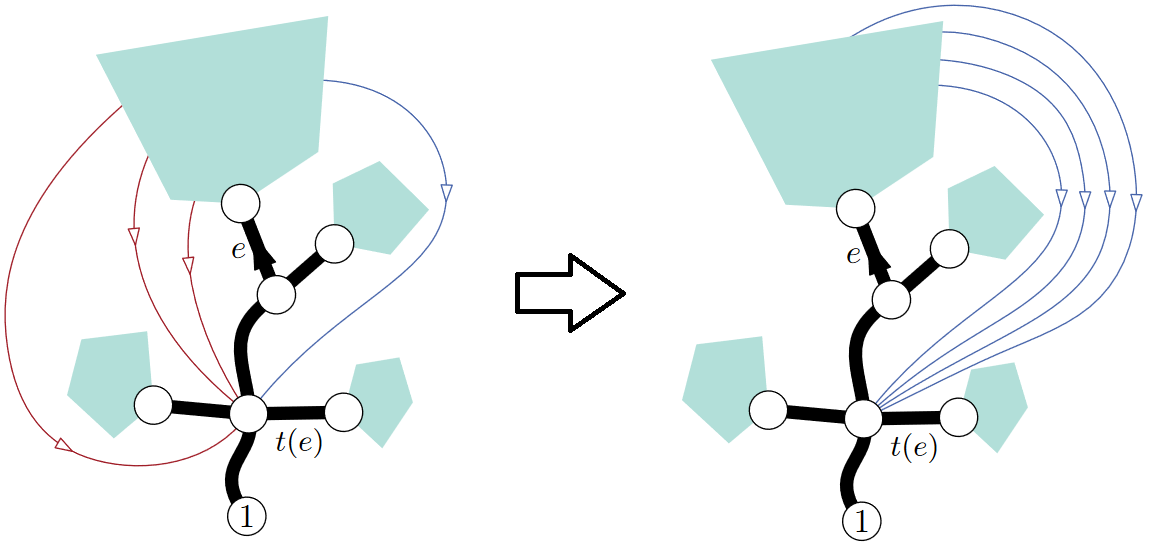
\includegraphics[width=0.5\textwidth]{images/lr-3.png}
	\end{center}
\end{itemize}

\textbf{Schritt 2}: LR-Zerlegung auf Baumkanten erweitern
\begin{itemize}
	\item Sei $e = vw$ eine Baumkante. Betrachte Rückkante $e_H$ von $e$ deren Rückkehrpunkt die höchste DFS-Zahl hat, aber nicht $v$ ist
	\item Füge $e$ der Menge, in der $e_H$ ist, hinzu
	\begin{center}
		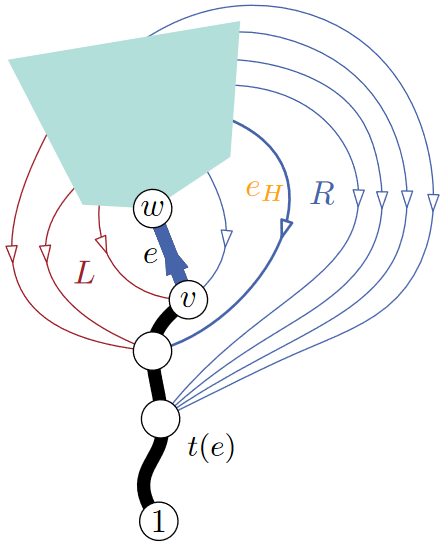
\includegraphics[width=0.2\textwidth]{images/lr-4.png}
	\end{center}
\end{itemize}

\textbf{Schritt 3}: Reihenfolge der ausgehenden Kanten festlegen
\begin{itemize}
	\item Für Knoten $v$ und ausgehende Kanten $e_1,e_2\in L$ definiere $e_1\prec e_2$ wenn
	\begin{itemize}
		\item entweder $t(e_2)<t(e_1)$
		\item oder $t(e_2)=t(e_1)$ und $e_1$ hat noch weiteren Rückkehrpunkt
	\end{itemize}
	\begin{center}
		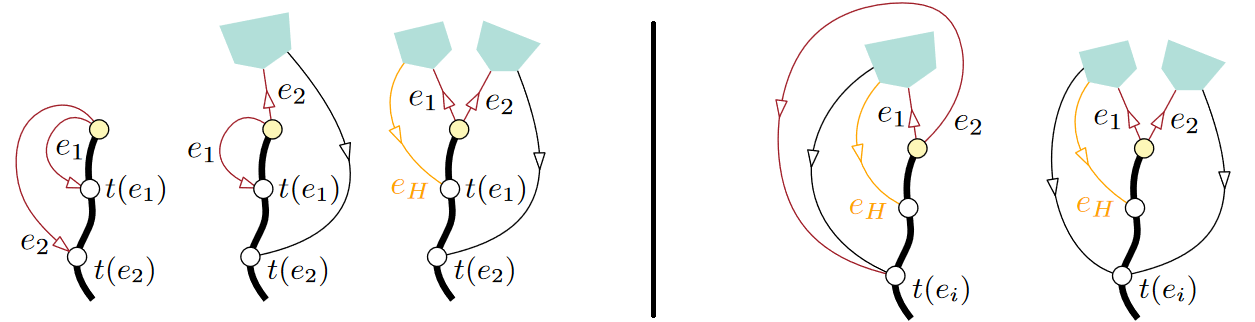
\includegraphics[width=0.55\textwidth]{images/lr-5.png}
	\end{center}
	\item Im Uhrzeigersinn ist die Ordnung der $L$-Kanten um $v$ dann $e_1^L\prec e_2^L\prec\cdots\prec e_l^L$
	\item $L$-Kanten sind also von innen nach außen sortiert
	\item Für $R$-Kanten ist die Sortierung genau andersrum
	\begin{center}
		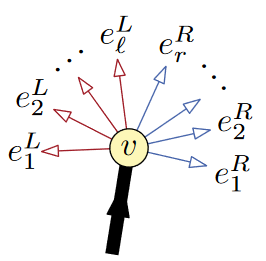
\includegraphics[width=0.15\textwidth]{images/lr-6.png}
	\end{center}
\end{itemize}

\textbf{Schritt 4}: Reihenfolge der eingehenden Kanten an v zur gleichen Baumkante $e=(v,w)$
\begin{itemize}
	\item Betrachte die eingehenden Kanten in $L$: $$L(e)=\{\text{Rückkante von }e\text{ eingehend an }v\}\cap L$$
	\begin{center}
		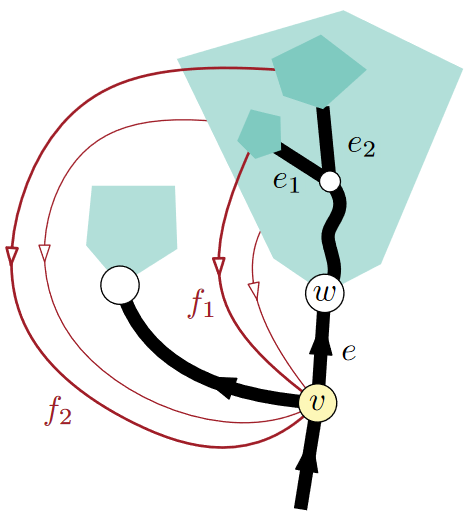
\includegraphics[width=0.2\textwidth]{images/lr-7.png}
	\end{center}
	\item Je zwei $f_1,f_2\in L(e)$ kommen von einer Gabel $e_1,e_2$, wobei $f_i$ Rückkante von $e_i$ ist
	\item Aus Schritt 3 haben die Kanten eine Ordnung bezüglich $\prec$ am Gabelknoten. O.B.d.A. sei nun $e_1\prec e_2$
	\item Setze dann $f_2\prec f_1$ an $v$, also genau umgekehrt
	\item Verfahre genauso für eingehende Kanten in $R$
\end{itemize}

\textbf{Schritt 5}: Inzidente Kanten an $v$ zyklisch sortieren
\begin{itemize}
	\item $e_1^L,\ldots,e_l^L,e_r^R,\ldots,e_1^R$ sortierte ausgehende Kanten
	\item Betrachte $L(e_i^L), R(e_i^L)$ bzw. $L(e_j^R), R(e_j^R)$ mit in Schritt 4 festgelegten Reihenfolge
	\item Für Nichtbaumkanten $e_i^L,e_j^R$ sind diese Mengen leer
	\item Definiere nun die Reihenfolge im Uhrzeigersinn an $v$ als:
	$$(u,v),L(e_1^L),e_1^L,R(e_1^L),\ldots,L(e_1^R),e_1^R,R(e_1^R)$$
	\begin{center}
		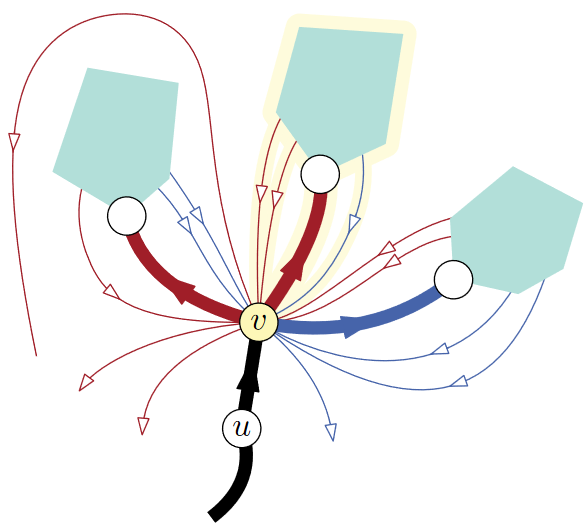
\includegraphics[width=0.25\textwidth]{images/lr-8.png}
	\end{center}
\end{itemize}

Dieser ganze Prozess kann in $\mathcal{O}(n)$ durchgeführt werden.